\documentclass[paper=a4, fontsize=11pt]{scrartcl} % A4 paper and 11pt font size
\usepackage{./../usfassignment}
\settitle{Assignment 8}
\setauthor{Wanzhang Sheng}
\setcourse{CS675: Automato Theory}

\begin{document}

\maketitle % Print the title

% -----------------------------------------------------------------------------
% PROBLEM 1
% -----------------------------------------------------------------------------
\section{}

\begin{fancyquotes}
  Give a 1-counter machine for each of the following languages.
\end{fancyquotes}

\begin{enumerate}
\item
  \begin{fancyquotes}
    (5 points) $L=$ all strings in ${(a+b+c)}^{*}$ that have the same
    number of $a$s as $b$s.
  \end{fancyquotes}

  \begin{figure}[hp]
    \centering
    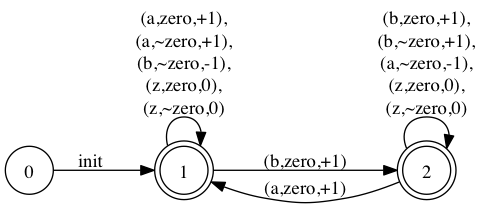
\includegraphics[width=.5\textwidth]{8-1.gv.png}
  \end{figure}

\item
  \begin{fancyquotes}
    (5 points) $L = \{a^{n}b^{3n}\}$.
  \end{fancyquotes}

  \begin{figure}[hp]
    \centering
    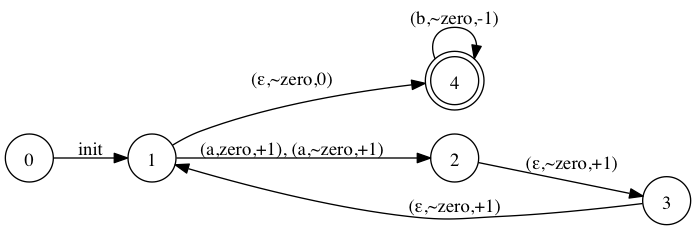
\includegraphics[width=.7\textwidth]{8-1.gv.2.png}
  \end{figure}

\end{enumerate}

\pagebreak

% -----------------------------------------------------------------------------
% PROBLEM 2
% -----------------------------------------------------------------------------
\section{}

\begin{fancyquotes}
  Show that the following functions are primitive recursive.
  You may define any helper functions that you wish.
  Eficiency is not a concern.
\end{fancyquotes}

\begin{enumerate}
\item
  \begin{fancyquotes}
    (5 points) $\gcd(m, n)$, the greatest common divisor of
    $m$ and $n$
  \end{fancyquotes}

  \begin{equation}
    \mathit{if}(c,t,e) = \mathit{add}(\mathit{mult}(t,\mathit{iszero}(\mathit{iszero}(c))), \mathit{mult}(e,\mathit{iszero}(c)))
  \end{equation}

  \begin{equation}
    \mathit{min}(a,b) = \mathit{if}(\mathit{iszero}(\mathit{sub}(m,n)), a, b)
  \end{equation}

  \begin{equation}
    \mathit{check}(m,n,k) = \mathit{and}(\mathit{iszero}(\mathit{div}(m,k)), \mathit{iszero}(\mathit{div}(n,k)))
  \end{equation}

  \begin{equation}
    f(m,n,k) = \mathit{if}(\mathit{iszero}(\mathit{sub}(k,1)), 1, \mathit{if}(\mathit{check}(m,n,k), k, \mathit{find}(m, n, k-1)))
  \end{equation}

  \begin{equation}
    \mathit{gcd}(m,n) = f(m,n,\mathit{min}(m,n))
  \end{equation}

\item
  \begin{fancyquotes}
    (5 points) $\mathit{prime}(n)$, a predicate function that is true
    if $n$ is prime.
  \end{fancyquotes}

  \begin{equation}
    f(n,k) = if(\mathit{equal}(\mathit{mod}(n,k),0), 0, f(n,k-1))
  \end{equation}

  \begin{equation}
    \mathit{prime}(n) = f(n,n-1)
  \end{equation}

\end{enumerate}

%\pagebreak

% -----------------------------------------------------------------------------
% PROBLEM 3
% -----------------------------------------------------------------------------
\section{}

\begin{fancyquotes}
  (5 points) Let $p(n)$ be the $n$th prime number function.
  Show that $p(n)$ is $\mu$-recursive.
\end{fancyquotes}

\begin{equation}
  p(n) =
  \begin{cases}
    2 & n==0\\
    \mu m[and(\mathit{prime}(m), \mathit{gt}(m,p(n-1)))]
  \end{cases}
\end{equation}

\pagebreak

\end{document}
